\newacronym{sujeitoa}{s.a.}{sujeito a}
\chapter{Otimização}
\label{ch:otimizacao}

\section{O problema da otimização}

Segundo \citeonline{Haugen2018} normalmente problemas de otimização são apresentados
como problemas de minimização, como: "Encontre o valor ótimo de $x$ que minimize a
\textit{função objetivo} $f(x)$, levando em consideração qualquer restrição sobre $x$
ou em função de $x$. A solução ótima é indicada por
\simbolo{xopt}{$ x_{opt} $}{Valor ótimo de $x$ para minimizar $f(x)$}" \cite{Haugen2018}.

\citeonline{Haugen2018} ainda mostra que há várias formas de formular matematicamente
um problema de otimização (minimização), mas que de forma geral, dado um modelo
matemático $M$, é possível representá-lo como a minimização de $x$ para uma função
$f(x)$, ou seja:

\begin{equation}
	\min_{x} f(x)
\end{equation}

sujeto a (também denotado por "\acrshort{sujeitoa}") restrições, que podem ser na forma de:

\begin{itemize}
\item Restrições de desigualdade:
	\begin{equation}
		\label{eq:min_restr_desigualdade}
		g(x) \leq 0
	\end{equation}
	onde $g$ pode ser uma função linear ou não-linear.
	
\item Restrições de igualdade:
	\begin{equation}
		\label{eq:min_restr_igualdade}
		h(x) = 0
	\end{equation}
	onde $h$ pode ser uma função linear ou não-linear de $x$.
	
\item Limites superiores e inferiores
	\begin{equation}
		\label{eq:min_limites}
		x_{li} \leq x \leq x_{ls}
	\end{equation}
	Onde $li$ e $ls$ indicam `limite inferior' e `limite superior', respectivamente.
\end{itemize}

Sendo que as equações \ref{eq:min_restr_desigualdade} e \ref{eq:min_restr_igualdade}
definem restrições na relação entre as variáveis de otimização, enquanto
\ref{eq:min_limites} define as regiões limites destas mesmas variáveis.

Existem diversas métodos para encontrar a solução ótima para um problema de otimização
e a sessão a seguir irá mostrar exemplos e métodos numéricos simples que nos permitirão
entender em maiores detalhes como um problema de minimização pode ser resolvido. No
\cref{ch:mpc} faremos uso das minimizações para compreender como o \acrshort{mpc}
calcula valores ótimos dadas determinadas restrições em um dado horizonte de controle,
pois uma maior compreensão sobre problemas de minimização pode fazer grande diferença
no entendimento do controle \acrshort{mpc} em si.

\section{Algoritmos de otimização}

\subsection{Método de pesquisa em grade}

O método apresentado nesta sessão não aplicável a praticamente nenhum problema real
devido a sua ineficiência computacional, porém ele ajuda a ilustrar o objetivo de
todo o método numérico voltado para minimização.

Este método consiste em testar todos os valores de todas as variáveis (em um conjunto
de dados definido) para verificar qual combinação minimiza a função objetivo, ou seja,
testar todos os valores possíveis para $x(1)$, $x(2)$, $x(3)$, $...$, $x(n)$ com o
objetivo de encontrar o \gls{xopt}, valor de $x$ que minimiza $f$.

No caso de um único $x$, um laço condicional simples poderia testar todos os valores da
função objetivo. Para ilustrar essa ideia o código-fonte \ref{lst:grid_search_scalar}, em
Python, mostra como a função $f(x)$ abaixo poderia ser computada, caso o intervalo de
teste de $x$ fosse igual 100, ou seja, $N = 100$.

\begin{equation}
	\label{eq:grid_search_scalar}
	f(x) = 0,00232x^4 - 0,111x^3 + 1,8x^2 - 11,6x + 34,4
\end{equation}

Sendo que:
\[	2 \leq x \leq 22 \]

O intervalo $N = 100$ indica que serão analisados 100 valores entre $2$ e $22$.

\lstinputlisting[	
	caption={[Pesquisa em grade com número escalar]
			Pesquisa em grade com número escalar \\
		    Fonte: Autor},
	label={lst:grid_search_scalar},
	language=Python,
	style=Python_lang]
	{./4_Codes/grid_search_scalar.py}

A \cref{fig:grid_search_scalar} plotada a partir do código acima mostra,
destacado em vermelho, o valor de $x$ onde a $f(x)$ apresentava seu menor valor.
Repare que o gráfico apresenta dois vales distintos: um deles é o já mencionado
destaque em vermelho, onde o valor $x$ é $18,76$ e outro onde $x$ vale
aproximadamente $5,5$. O vale do gráfico onde o valor de $x$ produz o menor valor
de $f(x)$ é conhecido como \textit{mínimo global}, todos os outros são
\textit{mínimos locais}, pois são os valores mínimos da função apenas para uma
região limitada.

Algorítmos que buscam encontrar o valor mínimo de uma função podem erroneamente
convergir para mínimos locais. O método de pesquisa em grade não é um desses
algorítmos, pois ao verificar todos os valores de $x$ ele sempre encontrará o
valor de $x$ que minimiza a função objetivo, porém nas próximas sessões serão
apresentados métodos que, apesar de serem mais eficientes computacionalmente,
podem tender para mínimos locais.
	
\begin{figure}
	\begin{center}
		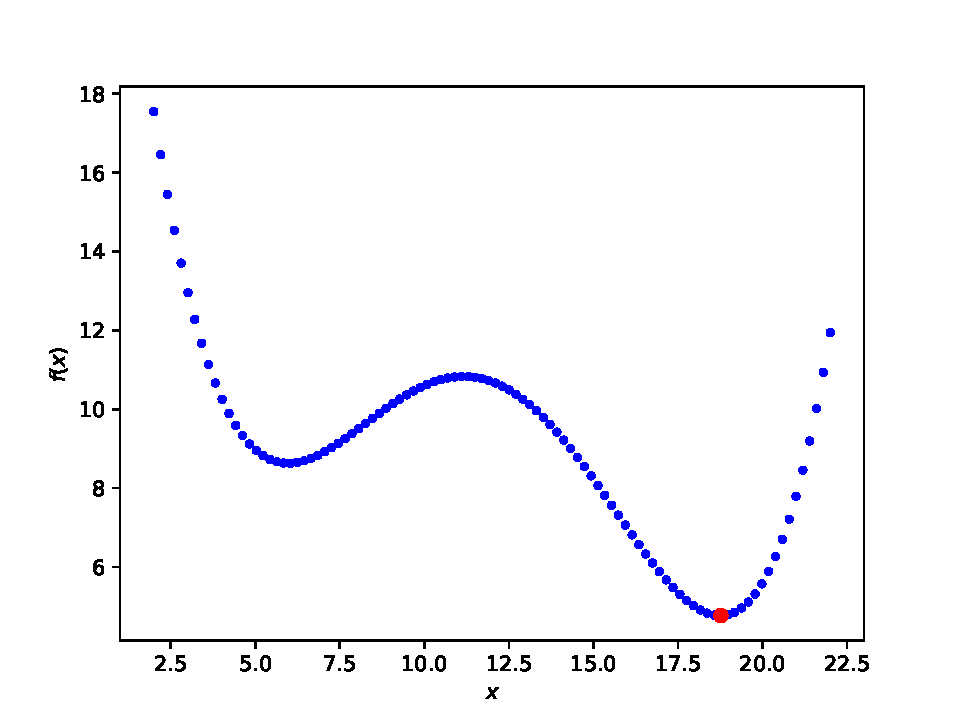
\includegraphics[width=0.8\textwidth]{./5_images/fig_grid_search_scalar.pdf} 
		\caption{Pesquisa em grade com número escalar}
		\label{fig:grid_search_scalar}
		\makebox[\width]{Fonte: Autor}
	\end{center}
\end{figure}

Ainda neste método, casos onde há uma maior quantidade de $x$ ($x_1$, $x_2$, \dots)
deve-se utilizar laços aninhados para que a varredura de todas as possibilidades
possa ser feita. 

Como exemplo, minimizemos a \cref{eq:grid_search_vect_no_bounds}, sendo
$0 \leq x_1 \leq 2$ e $1 \leq x_2 \leq 3$.

\begin{equation}
	\label{eq:grid_search_vect_no_bounds}
	f(x) = (x_1 - 1)^2 + (x_2 - 2)^2 + 0,5
\end{equation}

Neste caso, sem muito esforço notamos que
$f_{min} = 0,5$, $x_{1_{opt}} = 1$ e $x_{2_{opt}} = 2$.\footnote{
	O código-fonte em Python para este cálculo pode ser encontrado no
	\cref{ch:codigos_extras}, código \ref{lst:grid_search_vectorial}.}
Porém se a restrição da \cref{eq:grid_search_vect_bounds} for aplicada
encontramos os valores descritos nas equações descritas na \cref{eq:grid_search_vect_bounds_output}.

\begin{equation}
	\label{eq:grid_search_vect_bounds}
	f(x) = x_1 - x_2 + 1,5 \leq 0
\end{equation}

% \begin{subequations}
% 	\label{equ_grid_search_vect_bounds_output}
% 	\begin{align}
% 		f_{min} = 0,628 \\
% 		x_{1_{opt}} = 0,748 \\
% 		x_{2_{opt}} = 2,25
% 	\end{align}
% \end{subequations}

\begin{equation}
	\label{eq:grid_search_vect_bounds_output}
	\begin{aligned}
		f_{min} = 0,628 \\
		x_{1_{opt}} = 0,748 \\
		x_{2_{opt}} = 2,25
	\end{aligned}
\end{equation}

As figuras \ref{fig:grid_search_vectorial_nobounds} e \ref{fig:grid_search_vectorial_withbounds}
mostram a função custo (outra forma de chamarmos a função objetivo) sem restrição e com a
restrição descrita pela \cref{eq:min_restr_desigualdade}, respectivamente.

\begin{figure}[h]
    \centering
    \begin{minipage}{0.45\textwidth}
        \centering
        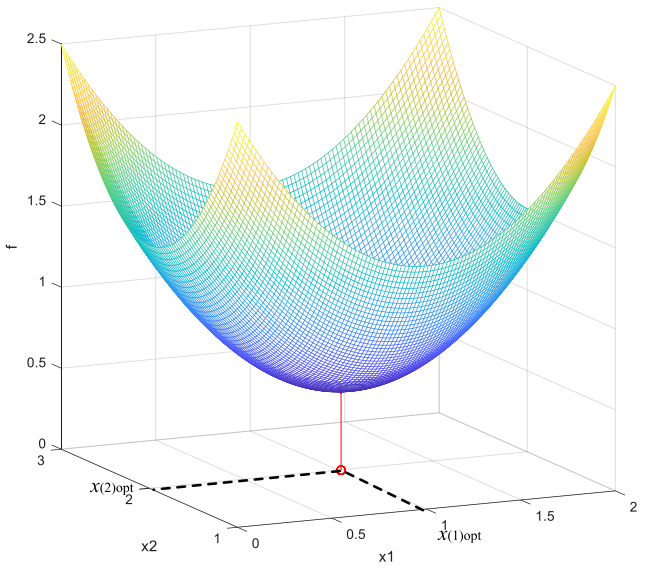
\includegraphics[width=0.9\textwidth]{./5_images/fig_grid_search_vectorial1.png} 
		\caption{Pesquisa em grade com duas variáveis e sem restrição}
		\label{fig:grid_search_vectorial_nobounds}
		Fonte: \citeonline{Haugen2018}
    \end{minipage}\hfill
    \begin{minipage}{0.45\textwidth}
        \centering
        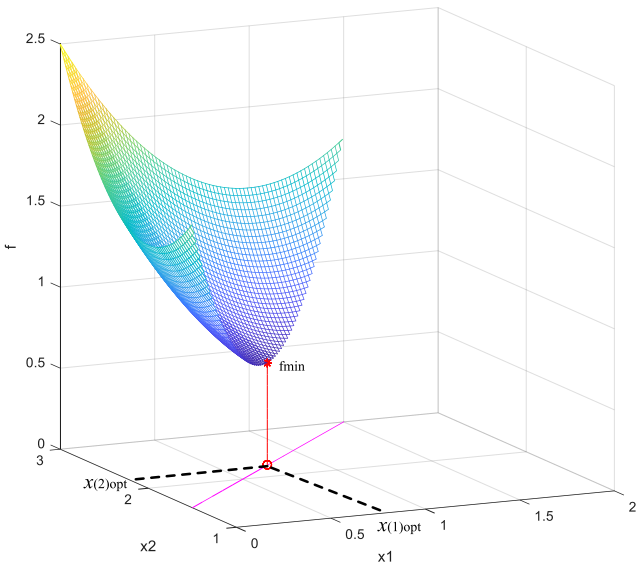
\includegraphics[width=0.9\textwidth]{./5_images/fig_grid_search_vectorial2.png} 
		\caption{Pesquisa em grade com duas variáveis e com restrição}  
		\label{fig:grid_search_vectorial_withbounds}		      
		Fonte: \citeonline{Haugen2018}
	\end{minipage}
\end{figure}

\subsection{Método de busca de descidas mais íngrimes}

Este método consiste em estimar o próximo valor de $x$ baseando-se na deriavada
da função custo calculada em $x$. Exemplificando para um caso escalar podemos dizer que
o próximo valor de $x$, isto é, $x_{k+1}$ será dado por:

\begin{align}
	\label{eq:steepest_decent_xk1}
	x_{k+1} &= x_k + \Delta x_k \\ 
	\Delta x_k &= -K f'(x_k)
\end{align}

\noindent
Onde: \\
$x_k$ = $x$ atual \\
$\Delta x_k$ = diferença entre $x_k$ e $x_{k+1}$ \\
$K$ = fator multiplicador do incremento \\
$f'(x_k)$ = derivada (ou gradiente) da função custo calculada em $x_k$ \newline

A derivada $f'(x_k)$ indica quão inclinada está a função custo no ponto $x_k$,
assim sendo o fator $K$ determina o peso que essa inclinação terá para o cálculo
do próximo valor de $x$.

A \cref{fig:steepest_decent_slope} mostra graficamente a influência da derivada
da função custo na amplitude de $\Delta x_k$ entre iterações.

\begin{figure}
	\begin{center}
		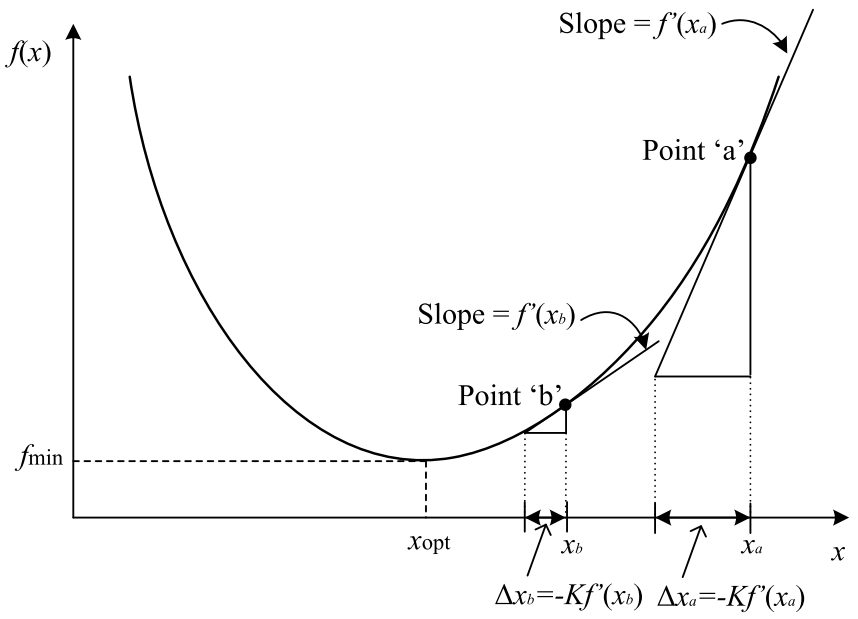
\includegraphics[width=0.75\textwidth]{./5_images/fig_steepest_decent_slope.png} 
		\caption{Influência de $f'(x_k)$ no cálculo de $x_{k+1}$ no método de descidas mais íngrimes}
		\label{fig:steepest_decent_slope}
		\makebox[\width]{Fonte: \citeonline{Haugen2018}}
	\end{center}
\end{figure}


\subsection{Método de Newton}

método de newton

\subsection{Otimizadores de programação não-linear (NLP)}

NLP

\section{Algumas aplicações de otimização}

\subsection{Estimação de parâmetros}

estimação de param

\subsection{Moving Horizon Estimation}

MHE

\subsection{Model Predictive Control}

MPC